\documentclass{ximera}

\colorlet{penColor}{blue!50!black} % Color of a curve in a plot
\colorlet{gridColor}{gray!50} % Color of grid in a plot
\colorlet{background}{white} % Color of the page


\outcome{Interpret real-word examples of limits via average velocity
  and instantaneous velocity}

\outcome{Interpert the slope of secant lines verses the slope of
  tangent lines.}

\outcome{Understand the difference between evaluating functions and
  taking limits of functions.}

\outcome{Using a graph to compute limits.}

\title{The idea of limits}

\begin{document}

\begin{abstract}
  This activity will motivate the need for limits in mathematics.
\end{abstract}
\maketitle

Limits appear in real world settings. In fact, your GPS device (or
phone) can use limits to estimate your velocity by computing
\textit{average velocity} on small time frames. You've known how to
compute average velocity for some time, it is just
\[
\text{average velocity} = \frac{\text{distance}}{\text{time}}.
\]
However, we are typically more interested in velocity at a specific
instant. This is called \textit{instantaneous velocity}.

\begin{question}
  %% Maybe a ball toss is better? 
  %% Not  sure. 
  Give a plot and ask about average velocities of smaller and smaller
  settings. Maybe driving from Columbus OH to Myrtle Beach SC. 
  \begin{image}
    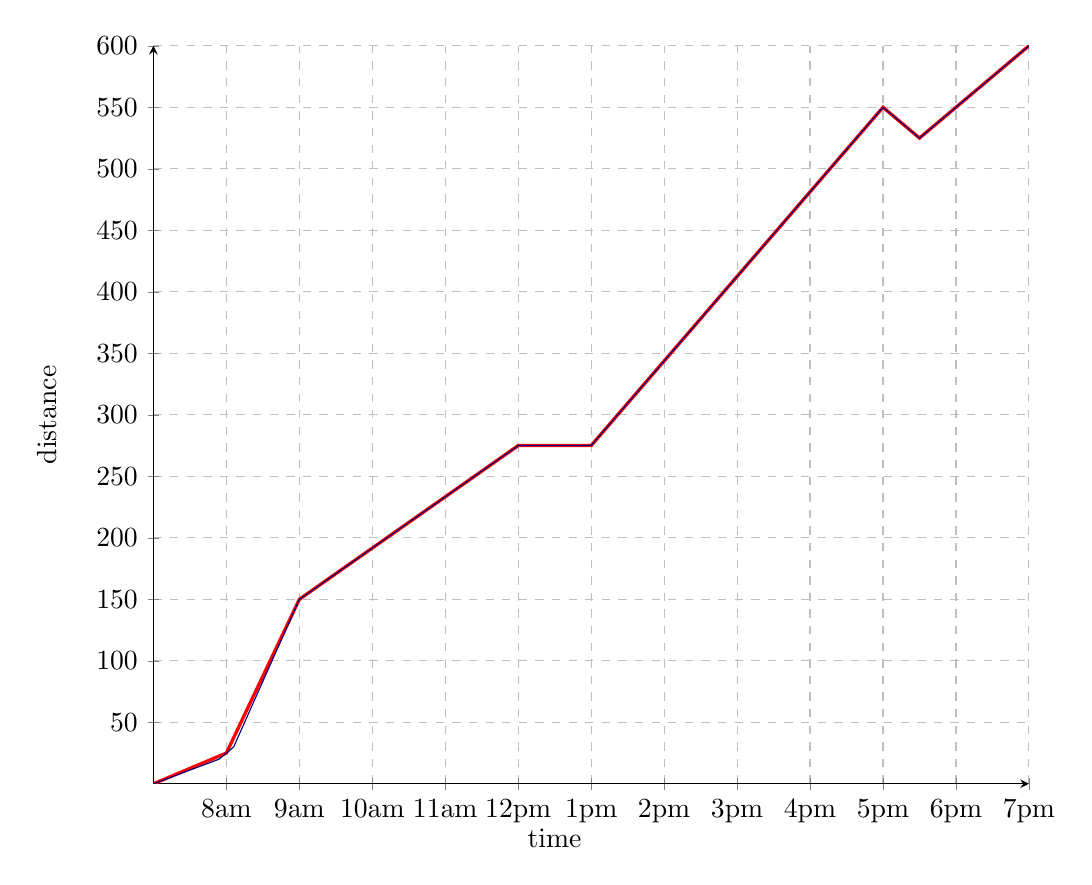
\begin{tikzpicture}
        \begin{axis}[
            xmin=0,
            xmax=12,
            ymin=0,
            ymax=600,
            width=5in,
            axis lines=middle,
            y label style={at={(axis description cs:-0.1,0.5)},rotate=90,anchor=south},
            x label style={at={(axis description cs:0.5,-0.1)}},
            xlabel=time, ylabel=distance,
            xtick={0,1,...,12},
            xticklabels={7am,8am,9am,10am,11am,12pm,1pm,2pm,3pm,4pm,5pm,6pm,7pm},
            ytick={0,50,...,600},
            grid=both,
            grid style={dashed, gridColor},
          ]
	  \addplot [very thick, red] coordinates {
            (0,0)
            (1,25)
            (2,150)
            (5,275)
            (6,275)
            (10,550)
            (10.5,525)
            (11,550)
            (12,600)
          };
	  \addplot [penColor] coordinates {
            (0,0)
            (.9,20)
            (1.1,30)
            (2,150)
            (5,275)
            (6,275)
            (10,550)
            (10.5,525)
            (11,550)
            (12,600)
          };
        \end{axis}
    \end{tikzpicture}
  \end{image}

  \begin{solution}
    \begin{multiple-choice}
      \choice[correct]{Correct answer}
      \choice{First Distractor}
      \choice{Second Distractor}
      \choice{Third Distractor}
    \end{multiple-choice}  
  \end{solution}
\end{question}

What other questions do you have about this lecture?
\begin{free-response}
Answers will vary.
\end{free-response}

\end{document}
